\section{Simulations:}

For each one of the circuits previously showed, a corresponding simulation was made, we capture the output voltage of the transformer {\bfseries\itshape $V_{T}$}, the Voltage in the $R_{L}$ resistor {\bfseries\itshape $V_{0}$} with and without filters and finally, the signal that corresponded to each circuit. Also all this information will be displayed in a table with the simulated circuit and his PSpice signal.

\subsection{Transformer:}

\begin{figure}[H]
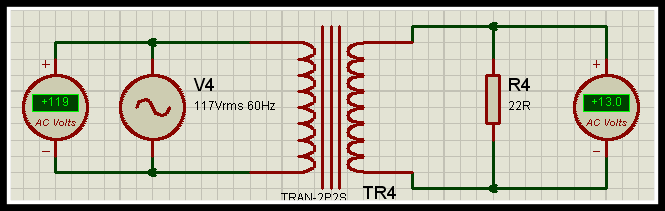
\includegraphics[scale=.63]{22RTransformer.png}
\centering \linebreak \linebreak Figure 4.1.0: Transformer with 22 $\Omega$ resistor.
\end{figure}

\begin{multicols}{2}
\begin{center}
\begin{tabular}[.5cm]{l c c}
\toprule
Resistor & $V_{rms}$ \\
\midrule
22 $\Omega$ & 13.0 $V$ \\
\bottomrule
\linebreak
\end{tabular}
\centering \linebreak Table 8: Measured values of Figure 4.1.0.
\end{center} \hfill

\end{multicols}

\begin{figure}[H]
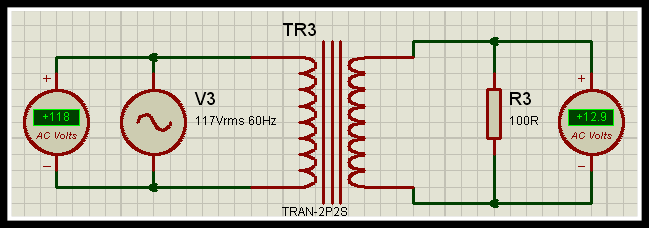
\includegraphics[scale=.64]{100RTransformer.png}
\centering \linebreak \linebreak Figure 4.1.1: Transformer with 100 $\Omega$ resistor.
\end{figure}

\begin{multicols}{2}
\begin{center}
\begin{tabular}[.5cm]{l c c}
\toprule
Resistor & $V_{rms}$ \\
\midrule
100 $\Omega$ & 12.9 $V$ \\
\bottomrule
\linebreak
\end{tabular}
\centering \linebreak Table 9: Measured values of Figure 4.1.1.
\end{center} \hfill

\end{multicols}

\pagebreak

\subsection{Half-Wave Rectifier:}

\begin{figure}[H]
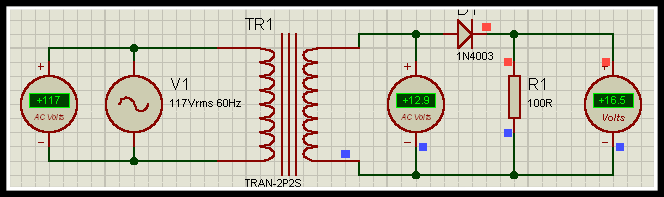
\includegraphics[scale=.63]{HW.png}
\centering \linebreak \linebreak Figure 4.2.0: Half-wave rectifier.
\end{figure}

\begin{multicols}{2}
\begin{center}
\begin{tabular}[.5cm]{l c c c}
\toprule
Resistor $R_{L}$ & $V_{T}$ & $V_{0}$ \\
\midrule
100 $\Omega$ & 12.9 $V$ &  16.5 V \\
\bottomrule
\linebreak
\end{tabular}
\centering \linebreak Table 10: Measured values of Figure 4.2.0.
\end{center} \hfill

\end{multicols}

\pagebreak

\subsection{Half-Wave Rectifier With Filter:}

\begin{figure}[H]
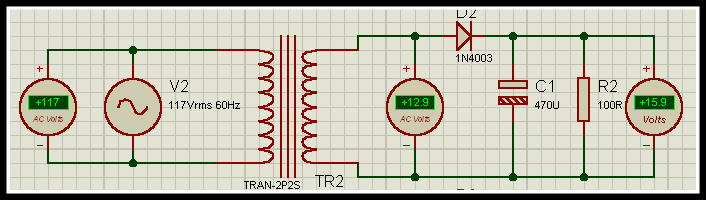
\includegraphics[scale=.59]{HW470F.png}
\centering \linebreak \linebreak Figure 4.3.0: Half-wave rectifier with 470 $\mu F$ capacitor.
\end{figure}

\begin{multicols}{2}
\begin{center}
\begin{tabular}[.5cm]{l c c c}
\toprule
Capacitor & $V_{T}$ & $V_{0}$ \\
\midrule
470 $\mu F$ & 12.9 $V$ &  15.9 V \\
\bottomrule
\linebreak
\end{tabular}
\centering \linebreak Table 11: Measured values of Figure 4.3.0.
\end{center} \hfill

\end{multicols}

\begin{figure}[H]
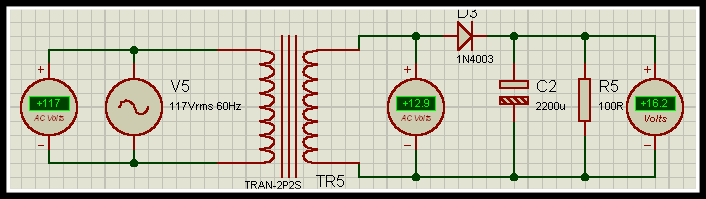
\includegraphics[scale=.59]{HW2200F.png}
\centering \linebreak \linebreak Figure 4.3.1: Half-wave rectifier with 2200 $\mu F$ capacitor.
\end{figure}

\begin{multicols}{2}
\begin{center}
\begin{tabular}[.5cm]{l c c c}
\toprule
Capacitor & $V_{T}$ & $V_{0}$ \\
\midrule
2200 $\mu F$ & 12.9 $V$ &  16.2 V \\
\bottomrule
\linebreak
\end{tabular}
\centering \linebreak Table 12: Measured values of Figure 4.3.1.
\end{center} \hfill

\end{multicols}

\pagebreak

\subsection{Full-Wave Center-Taped Rectifier:}

\begin{figure}[H]
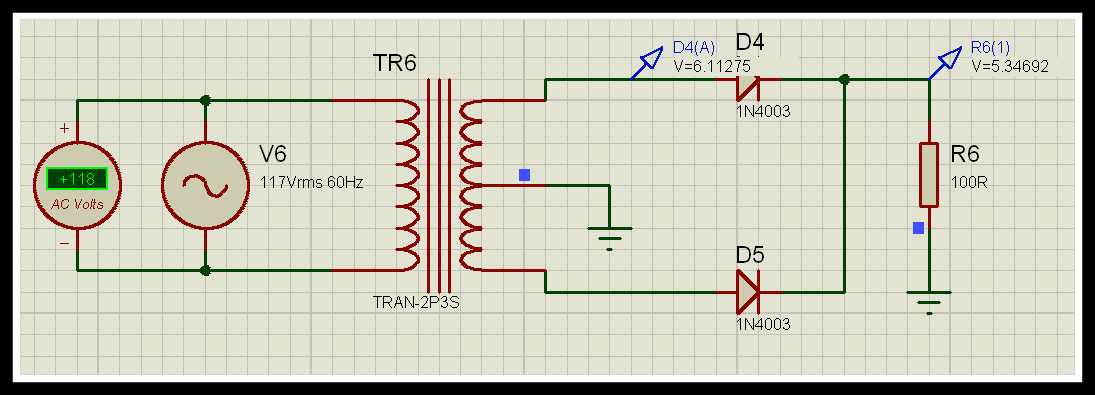
\includegraphics[scale=.38]{_FWCT.png}
\centering \linebreak \linebreak Figure 4.4.0: Full-wave center-taped rectifier.
\end{figure}

\begin{multicols}{2}
\begin{center}
\begin{tabular}[.5cm]{l c c c}
\toprule
Resistor $R_{L}$ & $V_{T}$ & $V_{0}$ \\
\midrule
100 $\Omega$ & 6.11 $V$ &  5.34 V \\
\bottomrule
\linebreak
\end{tabular}
\centering \linebreak Table 13: Measured values of Figure 4.4.0.
\end{center} \hfill

\end{multicols}

\pagebreak

\subsection{Full-Wave Center-Taped Rectifier With Filter::}

\begin{figure}[H]
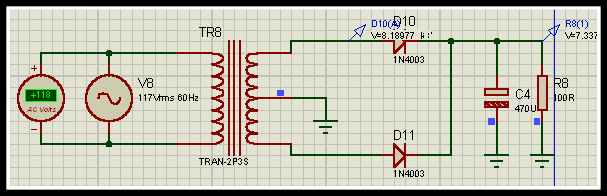
\includegraphics[scale=.68]{FWCT470F.png}
\centering \linebreak \linebreak Figure 4.5.0: Full-wave center-taped rectifier with 470 $\mu F$ capacitor.
\end{figure}

\begin{multicols}{2}
\begin{center}
\begin{tabular}[.5cm]{l c c c}
\toprule
Capacitor & $V_{T}$ & $V_{0}$ \\
\midrule
470 $\mu F$ & 8.1 $V$ &  7.3 V \\
\bottomrule
\linebreak
\end{tabular}
\centering \linebreak Table 14: Measured values of Figure 4.5.0.
\end{center} \hfill

\end{multicols}

\begin{figure}[H]
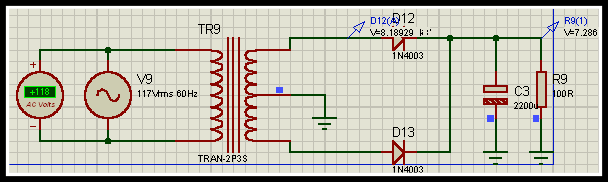
\includegraphics[scale=.68]{FWCT2200F.png}
\centering \linebreak \linebreak Figure 4.5.1: Full-wave center-taped rectifier with 2200 $\mu F$ capacitor.
\end{figure}

\begin{multicols}{2}
\begin{center}
\begin{tabular}[.5cm]{l c c c}
\toprule
Capacitor & $V_{T}$ & $V_{0}$ \\
\midrule
2200 $\mu F$ & 8.1 $V$ &  7.2 V \\
\bottomrule
\linebreak
\end{tabular}
\centering \linebreak Table 15: Measured values of Figure 4.5.1.
\end{center} \hfill

\end{multicols}

\pagebreak

\subsection{Full-Wave Bridge-Network Rectifier:}

\begin{figure}[H]
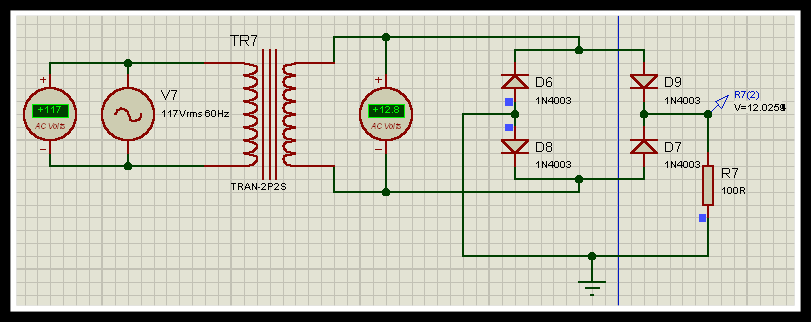
\includegraphics[scale=.505]{_FWBN.png}
\centering \linebreak \linebreak Figure 4.6.0: Full-wave bridge-network rectifier.
\end{figure}

\begin{multicols}{2}
\begin{center}
\begin{tabular}[.5cm]{l c c c}
\toprule
Resistor $R_{L}$ & $V_{T}$ & $V_{0}$ \\
\midrule
100 $\Omega$ & 12.8 $V$ &  12.02 V \\
\bottomrule
\linebreak
\end{tabular}
\centering \linebreak Table 16: Measured values of Figure 4.6.0.
\end{center} \hfill

\end{multicols}

\pagebreak

\subsection{Full-Wave Bridge-Network Rectifier With Filter::}

\begin{figure}[H]
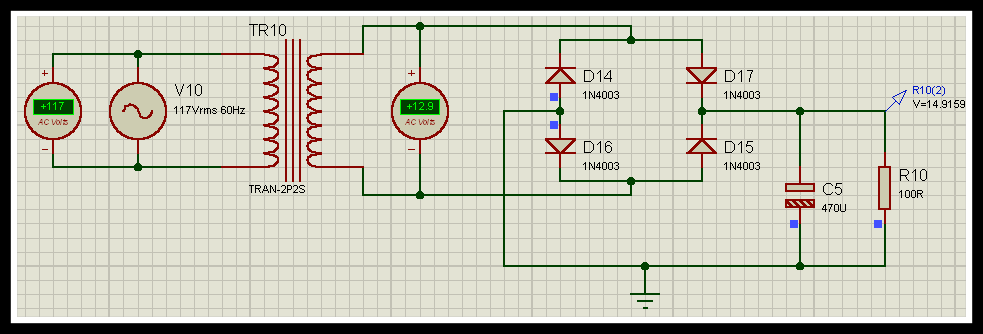
\includegraphics[scale=.42]{FWBN470F.png}
\centering \linebreak \linebreak Figure 4.7.0: Full-wave bridge-network rectifier with 470 $\mu F$ capacitor.
\end{figure}

\begin{multicols}{2}
\begin{center}
\begin{tabular}[.5cm]{l c c c}
\toprule
Capacitor & $V_{T}$ & $V_{0}$ \\
\midrule
470 $\mu F$ & 12.9 $V$ &  14.91 V \\
\bottomrule
\linebreak
\end{tabular}
\centering \linebreak Table 17: Measured values of Figure 4.7.0.
\end{center} \hfill

\end{multicols}

\begin{figure}[H]
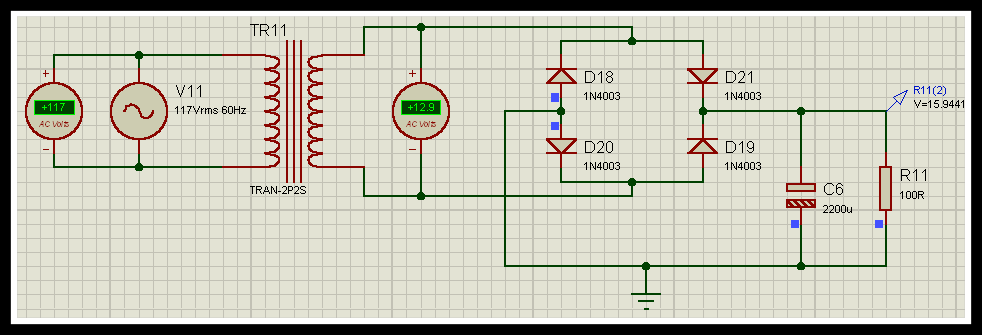
\includegraphics[scale=.42]{FWBN2200F.png}
\centering \linebreak \linebreak Figure 4.7.1: Full-wave bridge-network rectifier with 2200 $\mu F$ capacitor.
\end{figure}

\begin{multicols}{2}
\begin{center}
\begin{tabular}[.5cm]{l c c c}
\toprule
Capacitor & $V_{T}$ & $V_{0}$ \\
\midrule
2200 $\mu F$ & 12.9 $V$ &  15.94 V \\
\bottomrule
\linebreak
\end{tabular}
\centering \linebreak Table 18: Measured values of Figure 4.7.1.
\end{center} \hfill

\end{multicols}

\pagebreak